%%%%%%%%%%%%%%%%%%%%%%%%%%%%%%%%%%%%%%%%%%%%%%%
\chapter{Introduction and Motivation} \label{chap:introduction}
%%%%%%%%%%%%%%%%%%%%%%%%%%%%%%%%%%%%%%%%%%%%%%%

\section{The Era of Computing and Wireless Communication}
The ability to perform computations has evolved tremendously from the day the first computer was invented by Charles Babbage in the 19th century. By the end 19th century another important event occurred, in 1897 an Italian inventor and engineer Guglielmo Marconi demonstrated radio's ability to maintain continuous contact with ships in the English channel. A major breakthrough happened in the development of computers and wireless systems in 1948 when scientists at Bell Labs achieved groundbreaking results. Claude E.~Shannon published his paper \emph{``A mathematical theory of communication''}. John Bardeen, Walter Brattain, and William Shockley announced the invention of the \emph{transistor effect}. These two landmark events paved way for the widespread adoption of computers and wireless communication systems in numerous applications. Since then, the telecommunication industry has grown manifold fueled by the advancements in RF and transistor fabrication techniques, miniaturization and very large scale integration. These technological advances made computing devices smaller, cheaper and more reliable. Recent advances in wireless communication have allowed not only short distance communication such as cellular communication but also deep space communication with billions of kilometers distance.  \newline

Today computing devices and wireless systems have become integral parts of our society. They allow communication between people even from remote areas. The invention of the internet has enabled people to have access to a world of information in their fingertips. Until recently, wireless devices were primarily used for information exchange between people. Today's wireless applications are entering new avenues such as industrial automation, telemedicine, Autonomous driving. These applications demand ultra-reliability and ultra-low-latency. Latest mobile communication standard 5G took a giant step towards providing service for such mission-critical applications. 5G has adopted several techniques to service stringent latency requirements. To name few, different OFDM numerologies, flexible frame structure et cetera. Traditionally, to achieve stringent latency requirements wireless communication stacks are implemented in hardware, specifically in FPGAs/ASICs. Hardware implementations make use of implicit hardware-concurrency. However, hardware implementations come with inherent non-flexibility, huge cost and high development time. Due to the latest technological advancements in general-purpose computing, modern processors come with tremendous computation power. It is up to software engineer to efficiently harness this computational power. Modern processors come with special computing units to cater to specific application domains, namely vector processing units for signal processing applications. To achieve stringent latency requirements, it is very important that a software designer makes use of these additional processing elements and available optimization techniques. This work extensively makes use vector processing units through SSE, AVX and AVX2 instruction set extensions.

%Traditionally FEC chains are developed in hardware i.e FPGA’s or ASIC’s to achieve low latency and high throughput.
%Development in FPGA/hardware requires more time and costly.
%With recent advances in General Purpose Processors it is possible to achieve required latency and throughput with software implementations without custom hardware.
%Software implementations are flexible and easy to maintain compared hardware implementations.
%
%However algorithms need to be adopted/optimized to efficiently implement in software.
%
%Recent advances in the modern processors such as SIMD units can be utilized to achieve low latency and high throughput.

\section{Polar Forward Error Correction (FEC) Chain Development in Software}
Commonly high-performance signal processing and error correction applications are implemented in hardware either in FPGAs/ASICs. Hardware implementations allow these applications to achieve low latency and high throughput. Algorithms in these applications are developed targeting hardware implementations. These algorithms implemented in software without any reformulation or modification result in poor performance. Therefore algorithms need to be modified and reformulated to achieve expected performance in software. \newline

Optimizations for hardware such as recursive formulation, reducing look-up tables (LUTs) and flip-flops are not always relevant in software. Let's try to understand conflicts in the optimizations targeted for hardware and software. Most of the encoder/decoder algorithms are formulated in a recursive form. In hardware implementations, recursive formulations are particularly useful since same the design can be replicated multiple times without significant effort and also with no performance compromise. However, in software implementations recursive implementation incur with significant overhead. Mainly due to a large number of branches, stack allocation/deallocation, and pipeline flushing. The next optimization steps in hardware targeted implementations are minimizing the required memory and flip-flops. The cost of hardware implementation depends on the amount of memory and number flips-flops required\cite{minimizeFPGAResource}. In contrast, general-purpose computing world can make use of off-the-shelve available cheap memory. Software designer should reduce the number of cache misses and branch miss-predictions\cite{cacheMiss}. In addition, software implementations should also avoid expensive operations such as multiplications, division, and modulus operations. If not, reformulate them by using inexpensive bitwise operators. \newline

It is clear from above-discussed details that algorithms directly implemented in software without modification or reformulation result in poor performance. To achieve the best performance in software algorithms must be broken down into smaller operations mapped to specific functional units of modern processors. For example, a huge number of floating point/integer operations can be mapped to specialized vector processing units (SIMD) which are specifically designed to perform these operations. Mapping to vector processing units allows data parallelism. If an algorithm requires a lot of memory accesses, software should make use of special cache prefetching units to hide memory access latency. If a huge amount of data must be moved/copied based on previous decisions, such operations must be mapped to conditional move instructions and so forth.  Figure \ref{fig:operationMapping} gives visual illustration of mapping operations to specialized processing units/instructions.

\begin{figure}[]
	\centering
	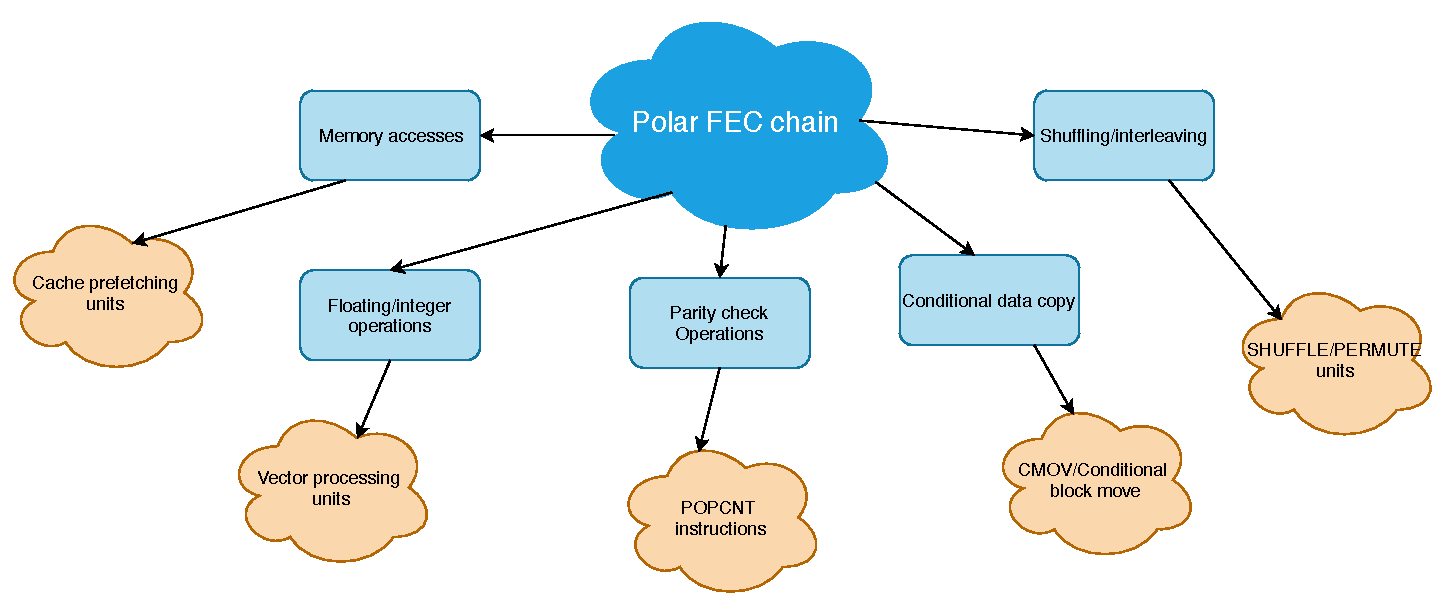
\includegraphics[width=1\textwidth]{./figures/operationMapping.pdf}
	\caption{Mapping FEC chain operations to particular functional units}
	\label{fig:operationMapping}
\end{figure}

This thesis work is a step in that direction. It tries to achieve maximum performance from modern general purpose processors to satisfy stringent latency requirements. The latest 3GPP standard has adopted polar codes for encoding and decoding control channel information \cite{3gpp.38.212}. Downlink control information (DCI) and Uplink control information (UCI) is transmitted using polar codes. In this work, polar encoding and decoding FEC chain are implemented in software. FEC chain algorithms are reformulated/optimized to suit a software implementation. FEC chain functionalities are broken down into primitive operations and mapped to specific computational units of general purpose processor. In this work, FEC chain implementation runs on a single processor core. The current implementation focuses on the off-the-shelf available AMD EPYC 7551P 32-Core general purpose processor\cite{amdEpyc}. It comes with state-of-the-art instruction extensions namely $\mathtt{SSE}$, $\mathtt{AVX}$, $\mathtt{AVX2}$ $\mathtt{3DNow!}$ et cetera. These advanced instructions allow mapping of different operations in FEC chain implementation to specialized processing units to maximize performance. 

Software implementation in this work makes extensive use of vector processing units, cache prefetching, branch prediction and compiler optimizations to achieve low latency. After the implementation, each component of the FEC chain performance of naive and optimized implementations are presented. At the end of encoding and decoding FEC chain chapters, overall latency of FEC chain is presented. Comparison between functional and optimized implementation is given to understand the importance of software optimizations. In decoding FEC chain chapter performance of implemented decoder is compared with state-of-the-art software decoder implementation\cite{lowLatencySWPolarDec}.

\section*{Organization of the Thesis}
Having described the overall problem and relevant motivation, in Chapter 2 the necessary background to develop polar FEC chain is provided. Including the required mathematical understanding of polar codes and fundamentals of modern computer architecture. In Chapter 3, Necessary details about different physical channels which use polar codes are presented. In Chapter 4, details of the polar encoding FEC chain are presented. Each component is analyzed for latency contribution. Both algorithmic and software optimizations are employed. In the end, the latency of naive and optimized implementations are compared. In Chapter 5, the details of polar decoding FEC chain are presented. Operation of different components in the FEC chain is given in detail. Each operation is optimized by mapping them efficiently to specific instructions/processing units. Decoder algorithm optimizations are presented and compared with state of the art software decoder implementations. Finally, at end of Chapter 5, the latency of the optimized decoding FEC chain is compared with the naive implementation.